% ============================================================
% SECTION 4: DASHBOARD
% ============================================================
\section{Dashboard OLAP}

% --- Slide 14 ---
\begin{frame}{Tổng quan Dashboard}
\begin{itemize}
  \item Xây dựng bằng \textbf{Streamlit} + \textbf{Plotly}, kết nối trực tiếp \texttt{airline\_dw.db}.
  \item \textbf{6 trang} điều hướng qua sidebar:
\end{itemize}

\vspace{2mm}
\small
\begin{table}
\centering
\begin{tabular}{clp{6.5cm}}
\toprule
\textbf{\#} & \textbf{Trang} & \textbf{Chức năng} \\
\midrule
1 & Tổng quan & KPI toàn ngành, cơ cấu chuyến, xu hướng delay \\
2 & Tuyến đường & Top tuyến theo hãng, lọc địa lý bang/sân bay \\
3 & Thời gian & Mùa vụ, thứ trong tuần, khung giờ bay \\
4 & Nguyên nhân & Cơ cấu delay, đóng góp tổng phút trễ \\
5 & Dự báo & Form nhập $\to$ xác suất delay thời gian thực \\
6 & Database Explorer & Schema, thống kê bảng, SQL tùy chỉnh \\
\bottomrule
\end{tabular}
\end{table}

\vspace{2mm}
Bộ lọc chung: \textbf{tháng/quý} + \textbf{hãng IATA} --- áp dụng cho 4 trang phân tích.
\end{frame}

% --- Slide 15 ---
\begin{frame}{Trang Tổng quan}
\begin{columns}[T,onlytextwidth]
\begin{column}{0.48\textwidth}
\textbf{5 KPI} (phản ứng theo bộ lọc):
\begin{itemize}
  \item Tổng chuyến bay: \textbf{5.332.914}
  \item OTP toàn ngành: \textbf{81,19\%}
  \item Tỉ lệ delay $\geq$15p: \textbf{18,81\%}
  \item Tỉ lệ hủy chuyến: \textbf{1,64\%}
  \item Delay trung bình: \textbf{4,8 phút}
\end{itemize}

\vspace{1mm}
\textbf{Biểu đồ:}
\begin{itemize}
  \item Cơ cấu chuyến bay theo tháng (cột chồng).
  \item Top 5 hãng OTP / Top 5 sân bay delay cao.
  \item Xu hướng delay \& hủy theo tháng.
\end{itemize}
\end{column}
\begin{column}{0.48\textwidth}
\centering
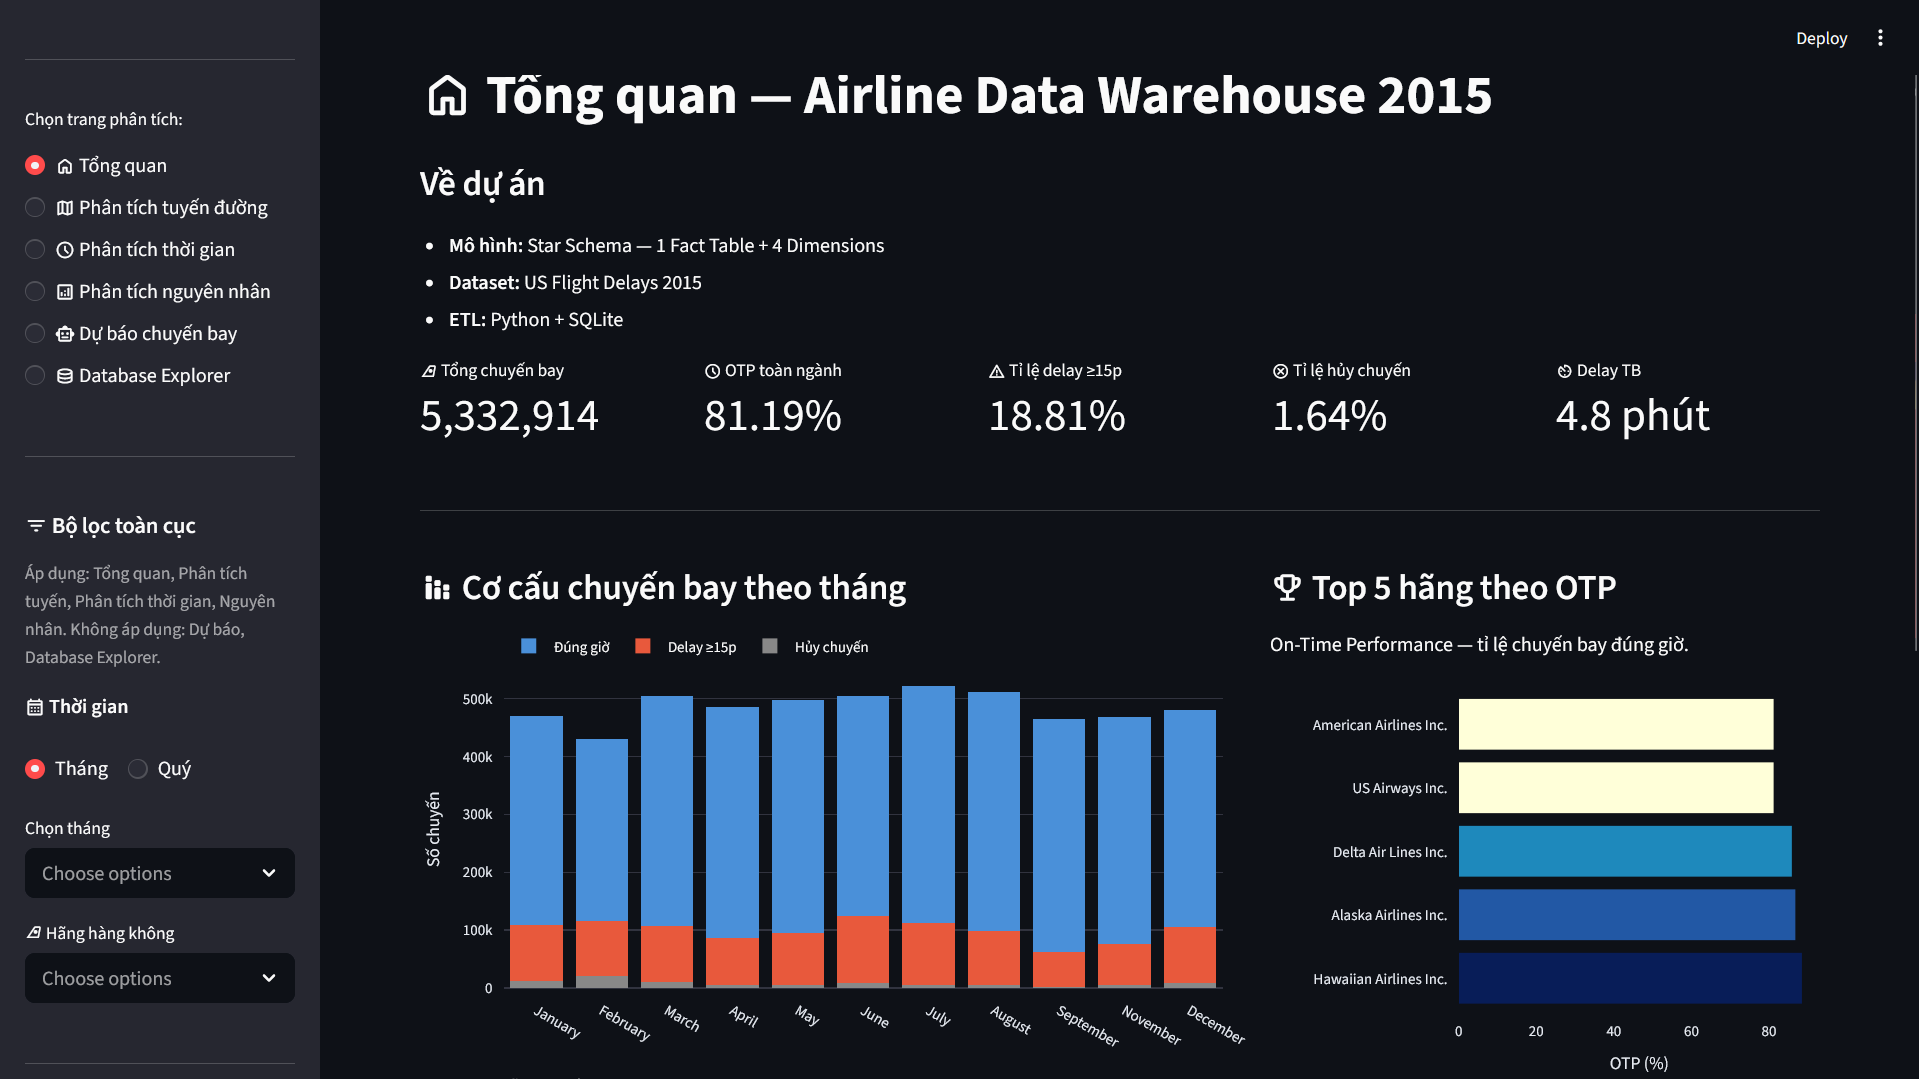
\includegraphics[width=\linewidth,height=0.7\textheight,keepaspectratio]{overview.png}
\end{column}
\end{columns}
\end{frame}

% --- Slide 16 ---
\begin{frame}{Trang Phân tích tuyến đường}
\begin{columns}[T,onlytextwidth]
\begin{column}{0.48\textwidth}
\begin{itemize}
  \item Top tuyến bay (cặp sân bay đi $\to$ đến) theo từng hãng.
  \item Bộ lọc địa lý: \textbf{bang xuất phát / bang đích},
        sau đó lọc tiếp theo sân bay cụ thể.
  \item Mỗi hãng sinh khối biểu đồ riêng,
        số tuyến và ngưỡng tối thiểu điều chỉnh được.
\end{itemize}
\end{column}
\begin{column}{0.48\textwidth}
\centering
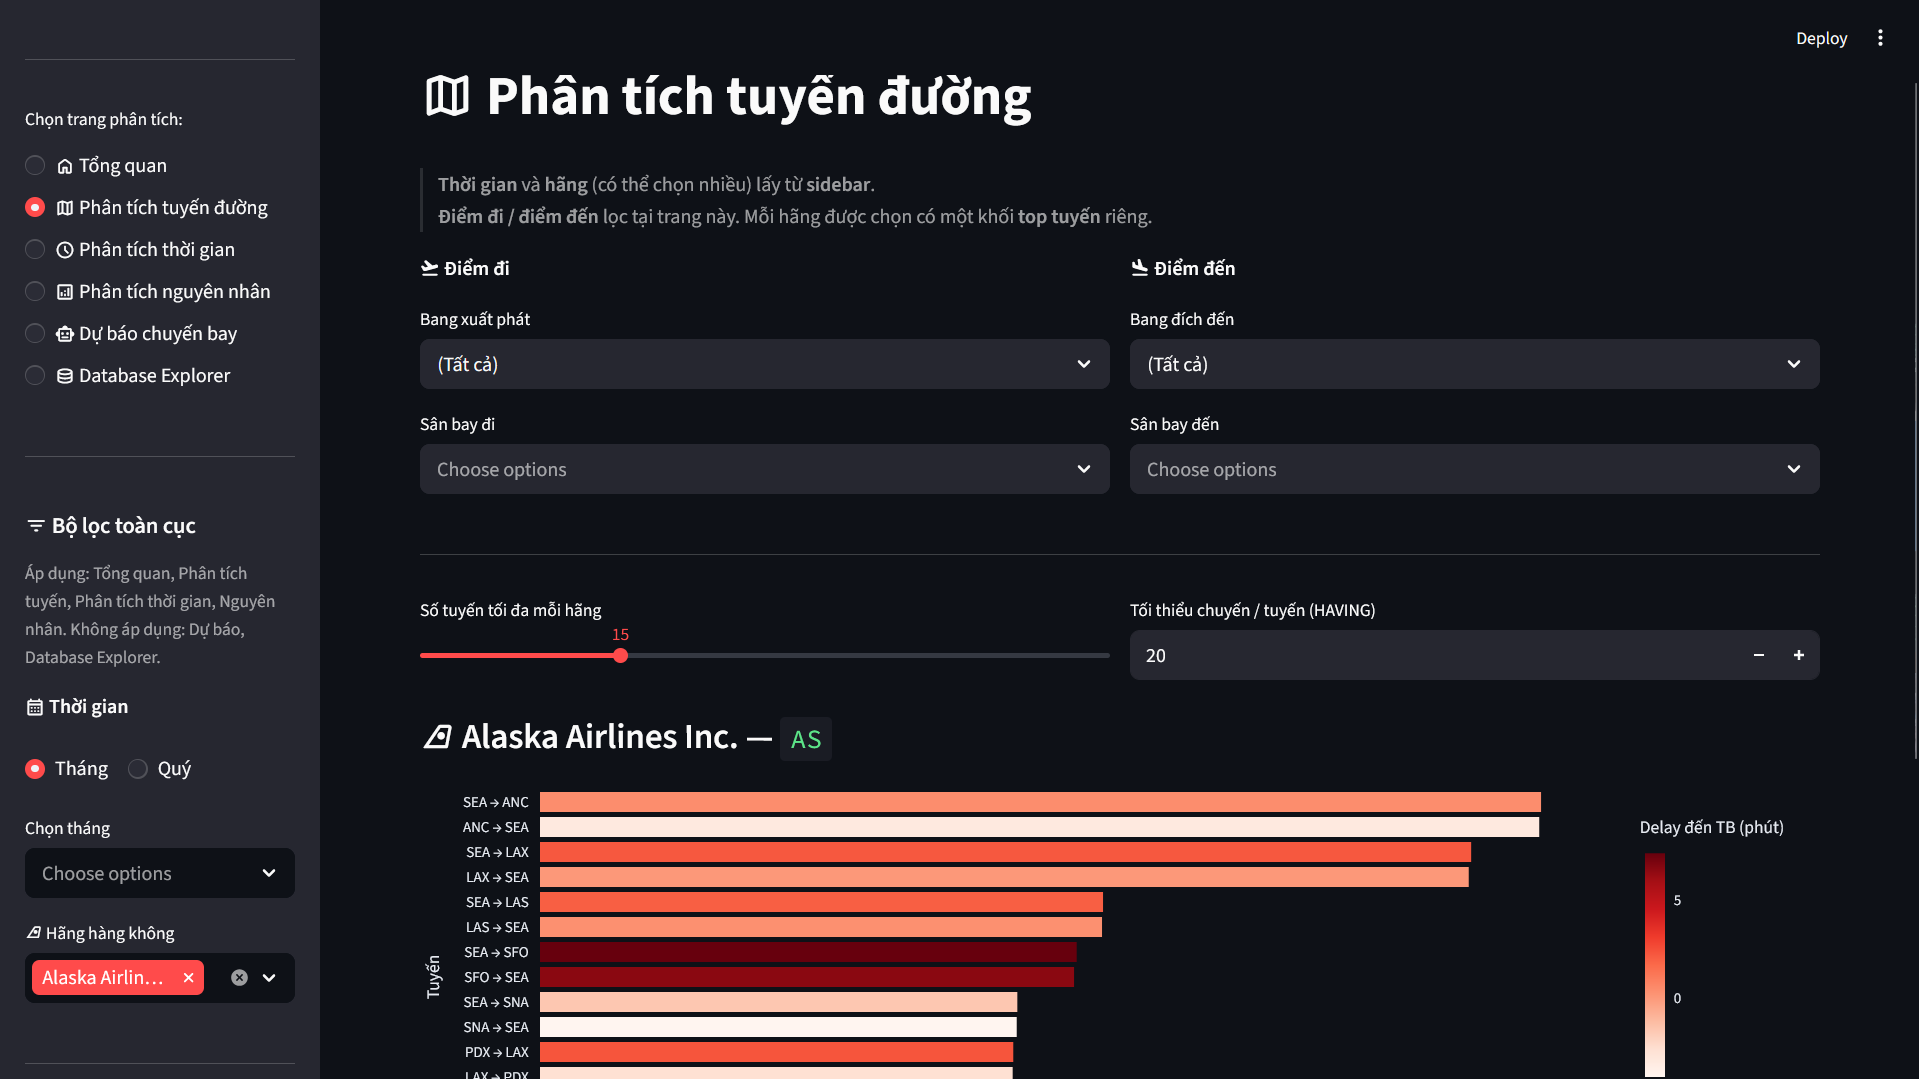
\includegraphics[width=\linewidth,height=0.7\textheight,keepaspectratio]{routes.png}
\end{column}
\end{columns}
\end{frame}

% --- Slide 17 ---
\begin{frame}{Trang Phân tích thời gian}
\begin{columns}[T,onlytextwidth]
\begin{column}{0.48\textwidth}
\begin{itemize}
  \item \textbf{Theo tháng}: heatmap số chuyến $\times$ nguyên nhân;
        delay TB tô màu theo mùa.
  \item \textbf{Theo quý}: cột delay TB Q1--Q4.
  \item \textbf{Theo thứ}: phút TB và tỷ lệ $\geq$15\%.
  \item So sánh ngày thường vs. cuối tuần:
        \textbf{5,4 phút} vs. \textbf{3,4 phút}.
  \item Delay theo \textbf{4 khung giờ} cất cánh.
\end{itemize}
\end{column}
\begin{column}{0.48\textwidth}
\centering
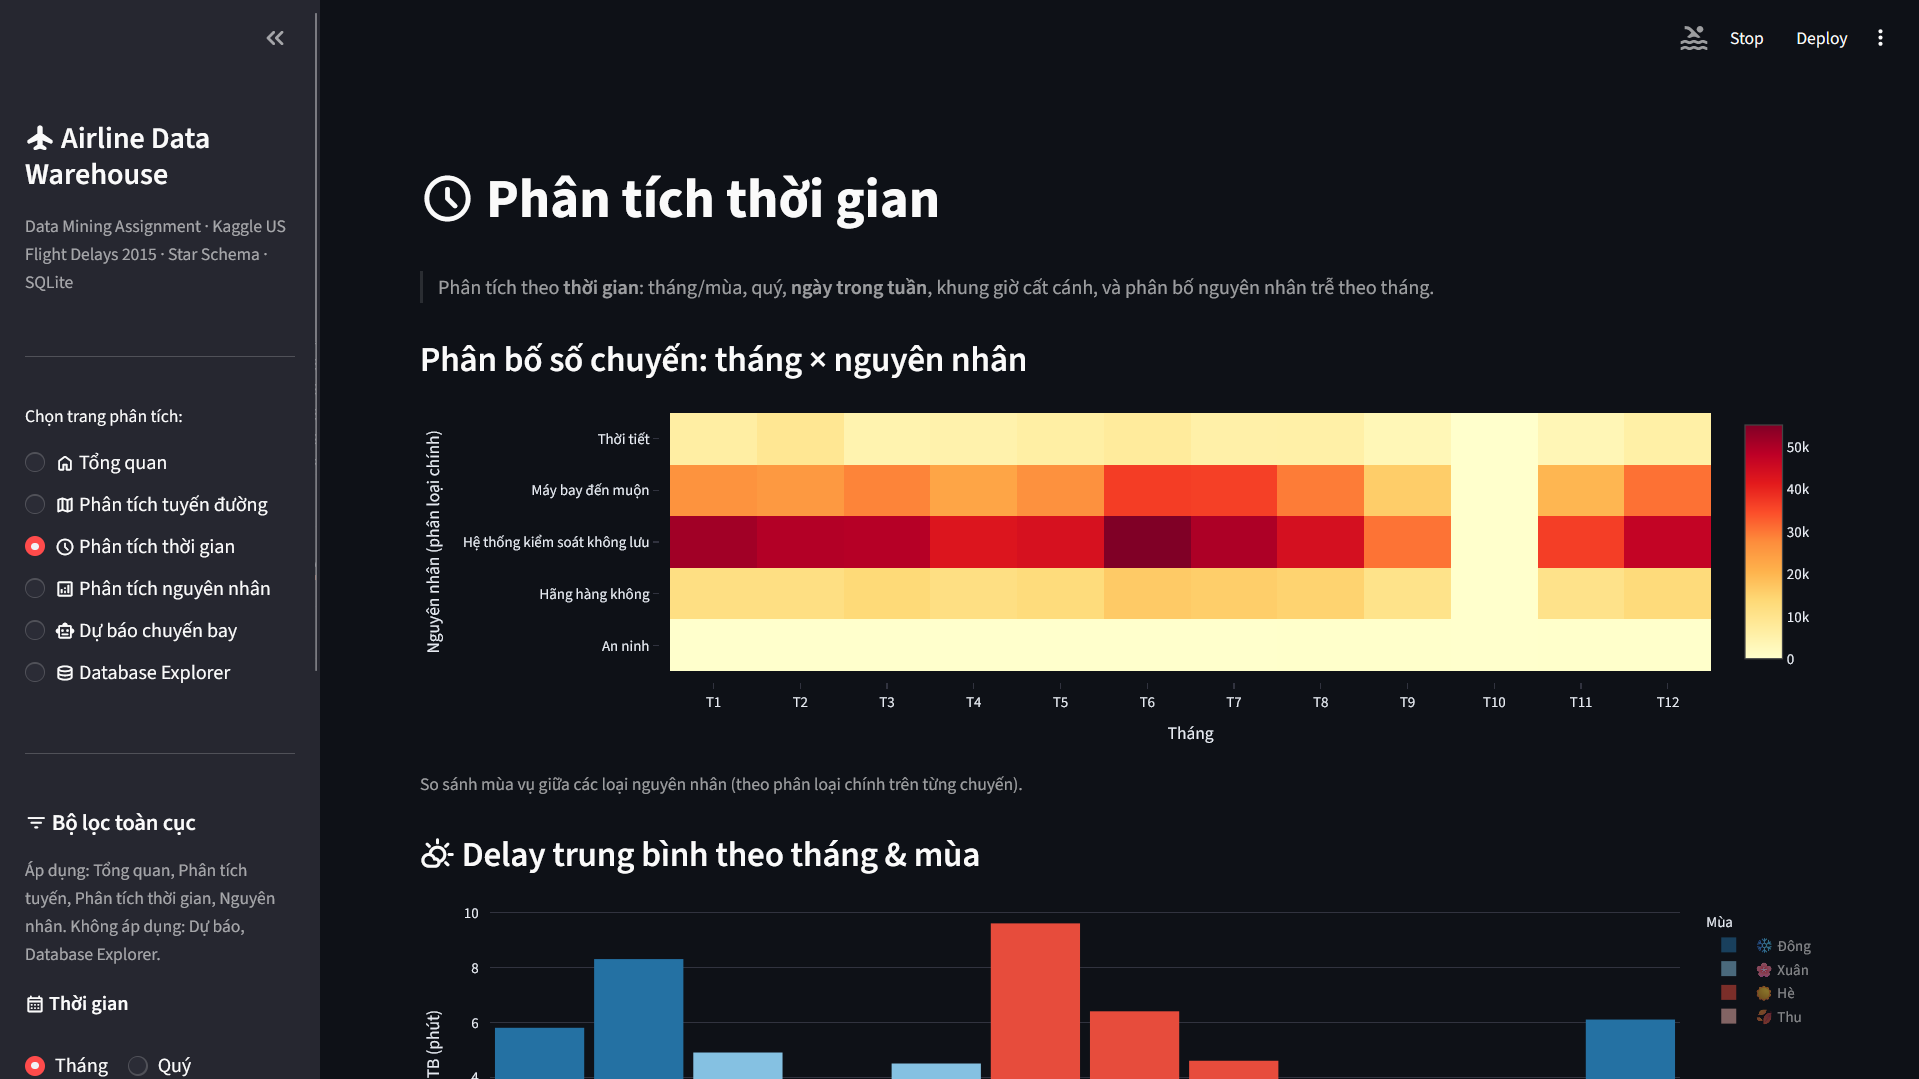
\includegraphics[width=\linewidth,height=0.7\textheight,keepaspectratio]{time.png}
\end{column}
\end{columns}
\end{frame}

% --- Slide 18 ---
\begin{frame}{Trang Phân tích nguyên nhân}
\begin{columns}[T,onlytextwidth]
\begin{column}{0.48\textwidth}
\begin{itemize}
  \item Pie cơ cấu số chuyến theo nguyên nhân.
  \item Cột ngang delay TB theo từng loại.
  \item Bảng tóm tắt: số chuyến, \%, delay TB, tổng phút trễ.
  \item Biểu đồ \textbf{đóng góp tổng phút trễ} --- nguyên nhân nào
        chiếm thời gian chờ lớn nhất?
\end{itemize}

\vspace{2mm}
\textbf{5 nguyên nhân:}\\
NAS, Late Aircraft, Carrier, Weather, Security.
\end{column}
\begin{column}{0.48\textwidth}
\centering
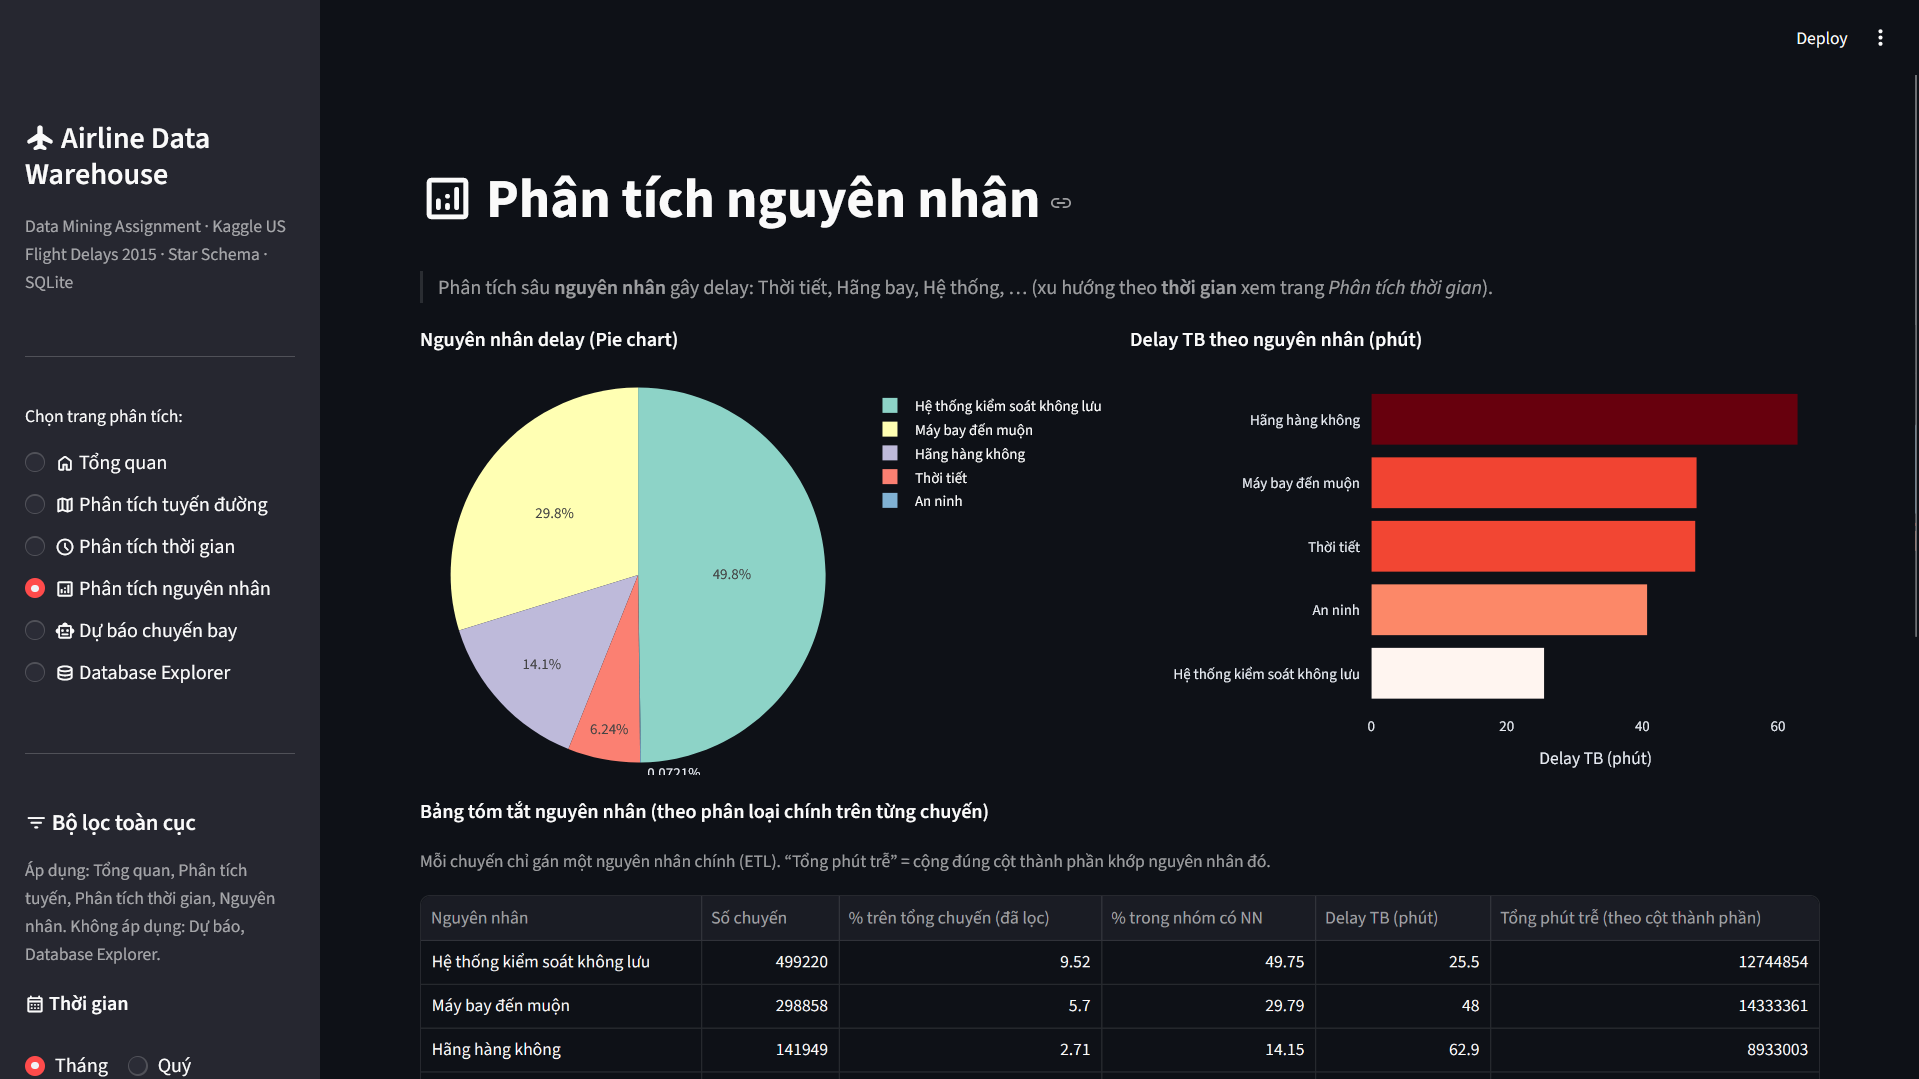
\includegraphics[width=\linewidth,height=0.7\textheight,keepaspectratio]{reason.png}
\end{column}
\end{columns}
\end{frame}

% --- Slide 19 ---
\begin{frame}{Trang Dự báo \& Database Explorer}
\begin{columns}[T,onlytextwidth]
\begin{column}{0.48\textwidth}
\centering
\textbf{Dự báo chuyến bay}\\[2mm]
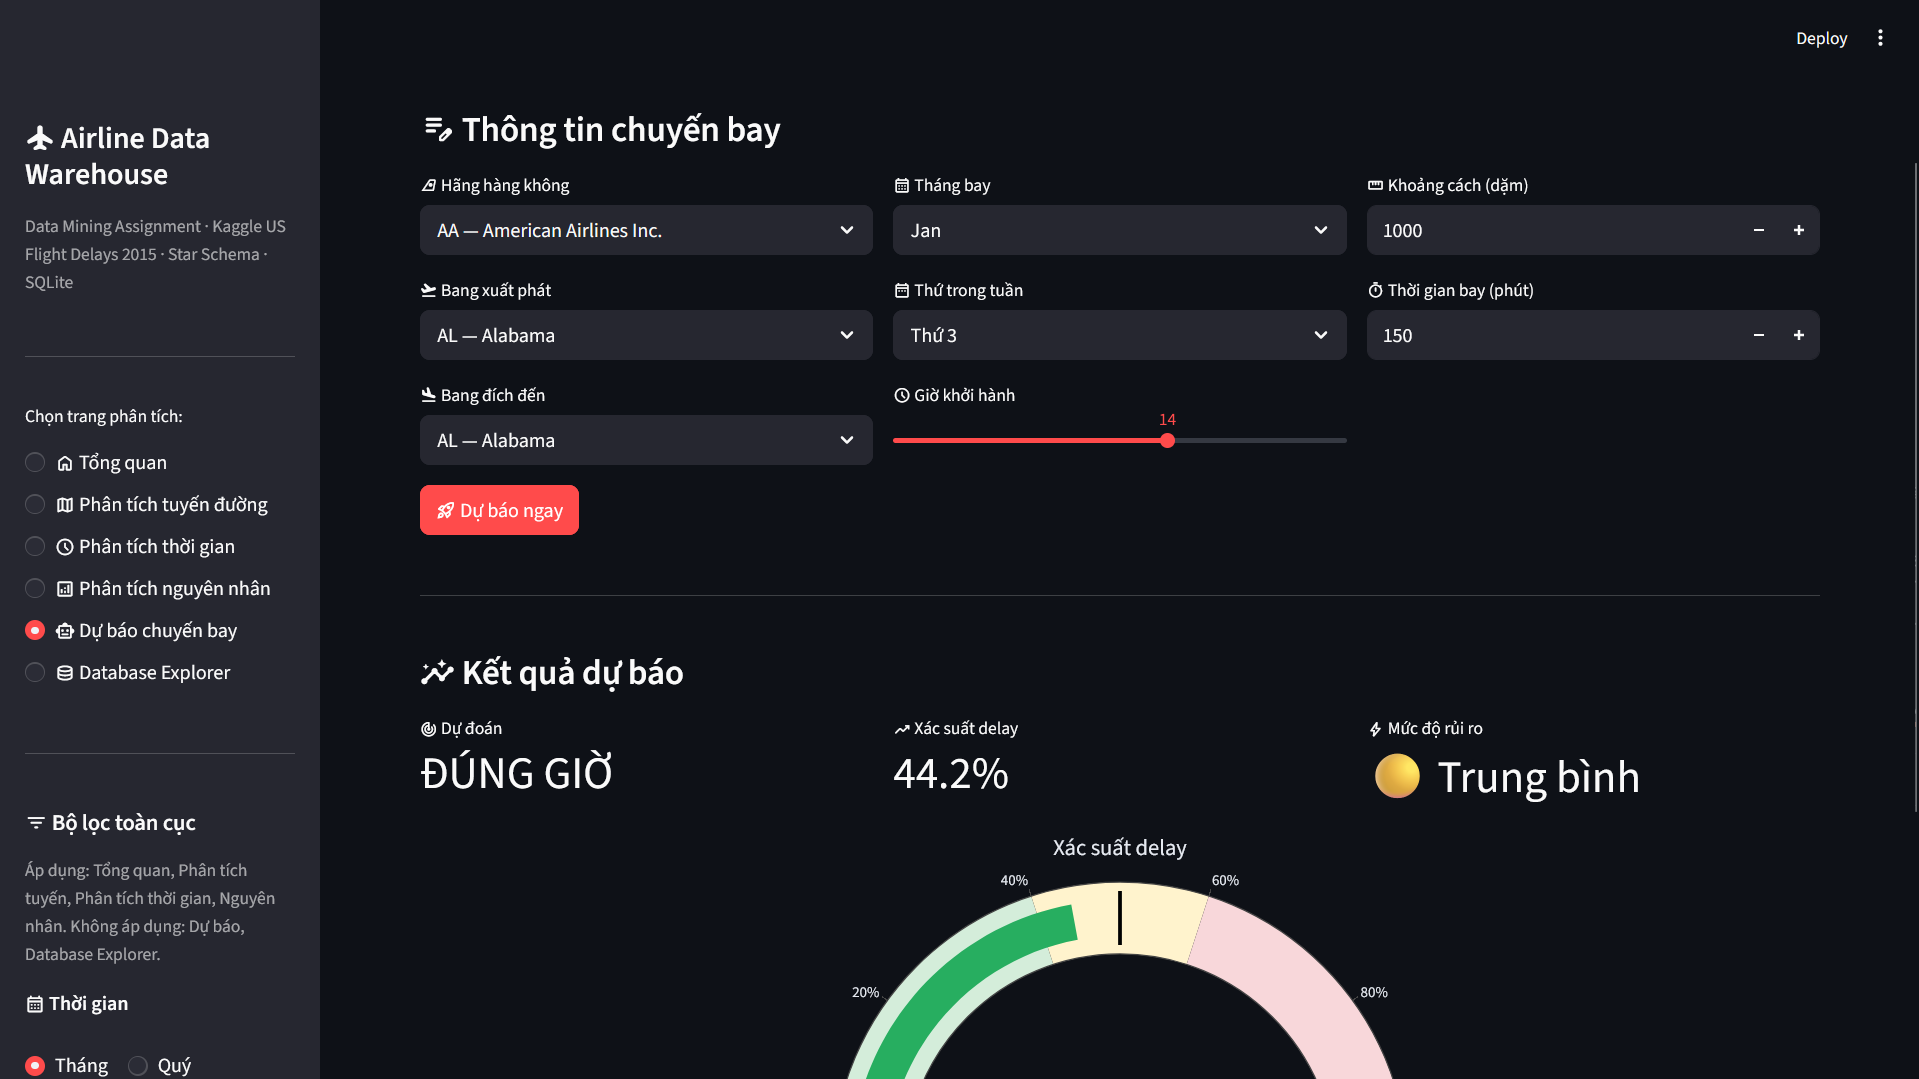
\includegraphics[width=\linewidth,height=0.48\textheight,keepaspectratio]{predict.png}\\
\scriptsize Form: hãng, bang đi/đến, tháng, thứ, giờ, distance, elapsed time
$\to$ nhãn + xác suất + gauge Plotly.
\end{column}
\begin{column}{0.48\textwidth}
\centering
\textbf{Database Explorer}\\[2mm]
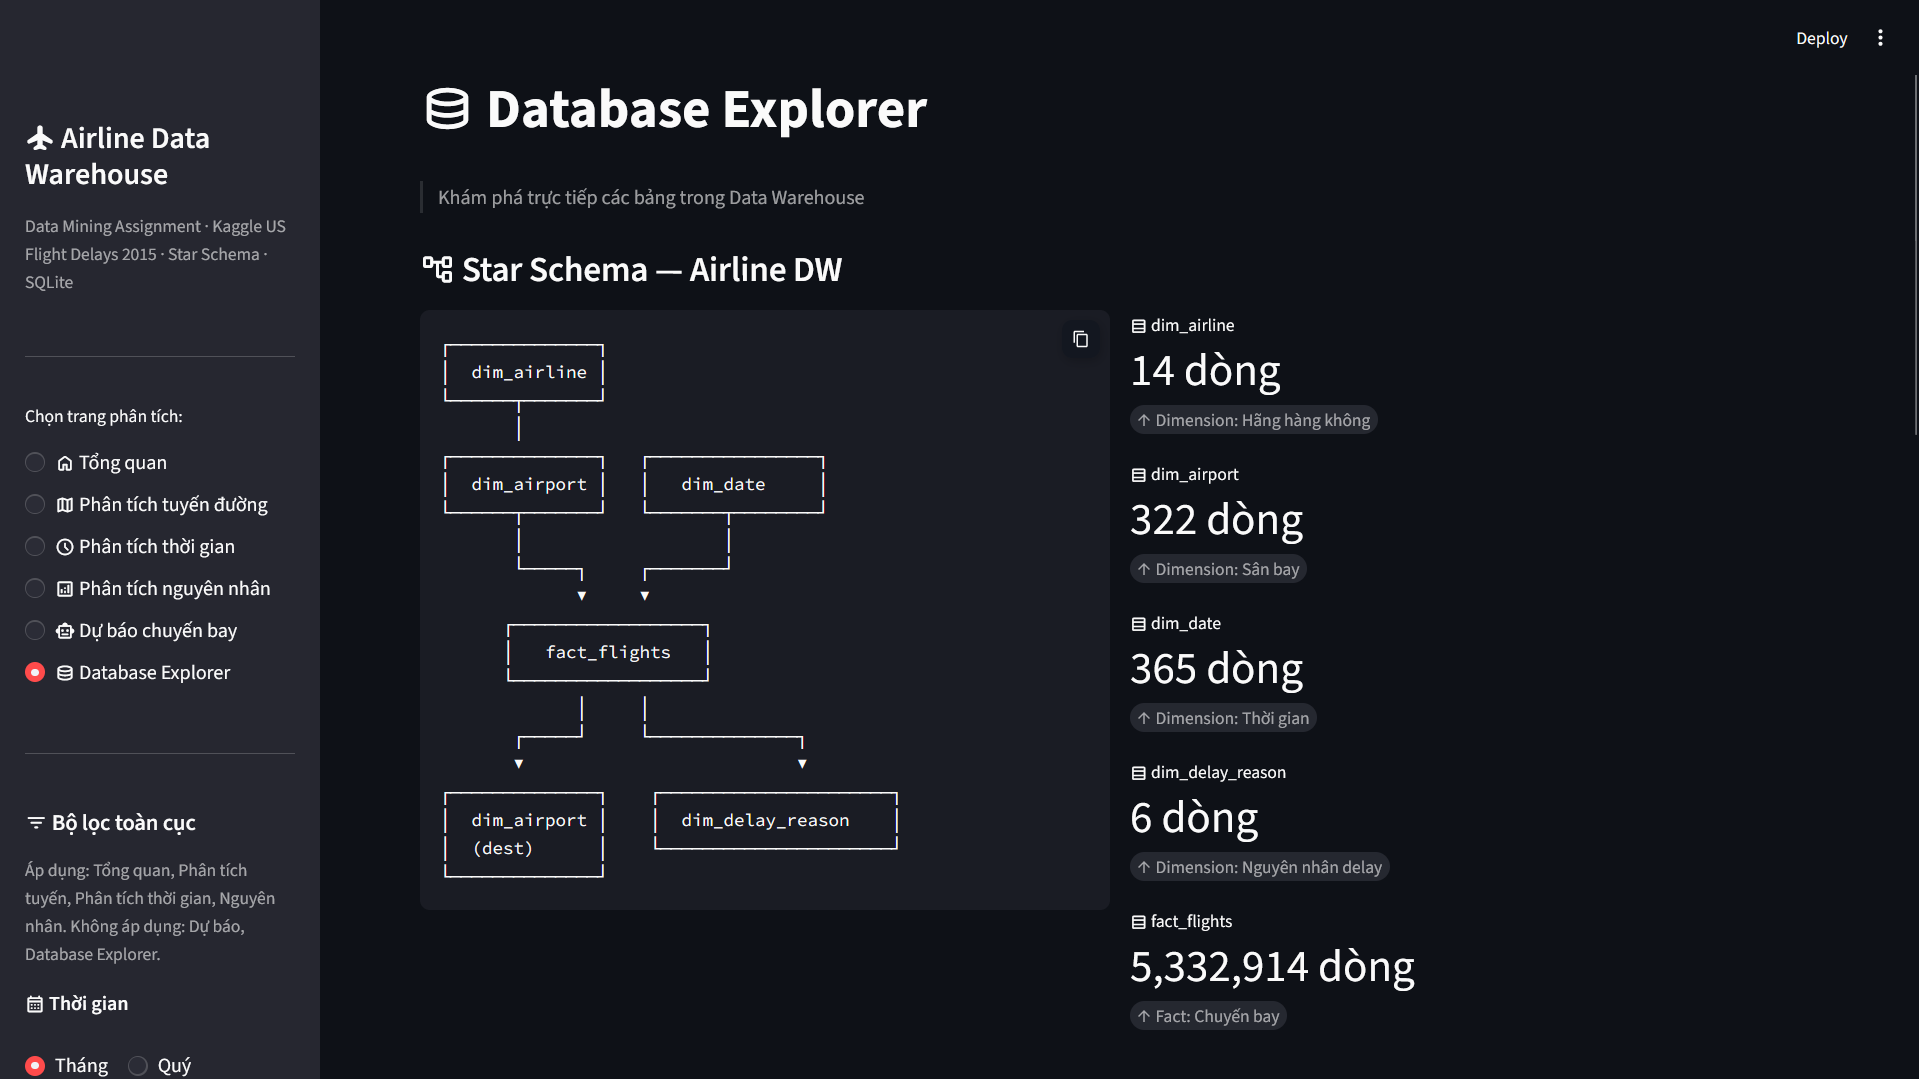
\includegraphics[width=\linewidth,height=0.48\textheight,keepaspectratio]{database.png}\\
\scriptsize Star schema ASCII, số dòng, xem trước bảng, SQL tùy chỉnh (chỉ SELECT).
\end{column}
\end{columns}
\end{frame}

% --- Slide 20 ---
\begin{frame}{Insight OLAP từ Dashboard}
Từ giao diện tương tác với dữ liệu năm 2015:

\begin{enumerate}
  \item \textbf{Tính mùa vụ rõ rệt:}
        Mùa hè (T6--T7) và mùa đông (T12--T1) là hai đỉnh delay.

  \item \textbf{Hiệu ứng tích lũy trong ngày:}
        Chuyến sáng sớm ($<$8h) ít delay nhất; chuyến tối chịu ảnh hưởng dây chuyền.

  \item \textbf{Chênh lệch giữa hãng:}
        OTP hãng tốt nhất vs. kém nhất chênh \textbf{15--20 điểm \%}.

  \item \textbf{Sân bay hub:}
        ORD, ATL, DFW có delay trung bình vượt mặt bằng chung.

  \item \textbf{Nguyên nhân chính:}
        NAS và Late Aircraft chiếm tỷ trọng trễ lớn nhất --- yếu tố \textit{hệ thống}.
\end{enumerate}
\end{frame}
